\documentclass[conference]{IEEEtran}
\usepackage{cite}
\usepackage{amsmath,amssymb,amsfonts}
\usepackage{graphicx}
\usepackage{textcomp}
\usepackage{xcolor}
\usepackage{booktabs}
\usepackage{tikz}
\usetikzlibrary{arrows.meta,positioning,shapes.geometric,fit}
\usepackage{pgfplots}
\pgfplotsset{compat=1.17}
\usepackage{url}
\usepackage{array}
\usepackage{placeins}
\usepackage{float}
\usepackage{algorithm}
\usepackage{algorithmic}
\usepackage[hidelinks,breaklinks=true]{hyperref}
\renewcommand{\dbltopfraction}{0.9}
\renewcommand{\dblfloatpagefraction}{0.7}
\setcounter{dbltopnumber}{2}

\def\BibTeX{{\rm B\kern-.05em{\sc i\kern-.025em b}\kern-.08em
    T\kern-.1667em\lower.7ex\hbox{E}\kern-.125emX}}

\begin{document}

\title{Agentic AI for Plant Disease Diagnosis: An Autonomous Multi-Agent Framework Integrating Vision, Retrieval, and Reasoning}

\author{
\IEEEauthorblockN{Lovepreet Sharma}
\IEEEauthorblockA{Department of Information Technology \\
Dr BR Ambedkar NIT Jalandhar \\
Jalandhar, Punjab, India \\
lovepreets.da.25@nitj.ac.in}
\and
\IEEEauthorblockN{Mithilesh Kumar Tiwari}
\IEEEauthorblockA{Department of Information Technology \\
Dr BR Ambedkar NIT Jalandhar \\
Jalandhar, Punjab, India \\
mithileshkt.da.25@nitj.ac.in}
\and
\IEEEauthorblockN{Jaspal Kaur Saini, IEEE Member}
\IEEEauthorblockA{Department of Information Technology,\\ Sports and Healthcare Research Centre \\
Dr BR Ambedkar NIT Jalandhar \\
Jalandhar, Punjab, India \\
{} corresponding author:\\ sainijk@nitj.ac.in, sainijassi87@gmail.com}
}

\maketitle

\begin{abstract}
Automated plant disease detection using convolutional neural networks has achieved strong classification accuracy on benchmark datasets such as PlantVillage, yet a standalone classifier provides only a label and a confidence score: it offers no explanation, no differential reasoning over plausible alternatives, and no mechanism to defer uncertain cases to a human expert. This paper presents an agentic artificial intelligence framework that wraps a ResNet-18 vision classifier with four cooperating agents: a Confidence and Image-Quality Agent, a Retrieval Agent, a Reasoning Agent, and an Orchestrator to convert disease classification into an autonomous, explainable, and safety-aware diagnostic advisory system. The Orchestrator grounds every actionable disease diagnosis in retrieved evidence, producing a cited treatment recommendation via the Reasoning Agent, while skipping this computation for healthy plants (which need no treatment) and escalating low-confidence, low-quality, or ambiguous inputs directly to human review rather than acting on them; prediction confidence and class ambiguity govern whether a recommendation is issued directly or accompanied by explicit caveats and alternatives. We evaluated the proposed system using both conventional classification metrics and a set of agentic metrics: correct-action rate, harmful-action rate, and human-intervention rate. On held-out PlantVillage images, individual models attain 86.0--99.1\% top-1 accuracy and the three-model federated ensemble (FedAvg, FedOpt, FedMA) matches the best single model at 99.1\%. These results support agent-orchestrated pipelines as a practical bridge between imperfect vision models and trustworthy, deployable agricultural decision support.
\end{abstract}

\begin{IEEEkeywords}
Agentic AI, Plant Disease Detection, Retrieval-Augmented Generation, Multi-Agent Systems, PlantVillage, ResNet-18, Precision Agriculture, Autonomous Decision-Making
\end{IEEEkeywords}

\section{Introduction}
\label{sec:intro}

Plant diseases remain a major threat to global food security, with pests and pathogens estimated to reduce yields by 20--40\% annually across major staple crops. Early and accurate diagnosis is essential because fungicide treatments and cultural interventions are most effective before disease reaches an advanced stage. Large, labeled visual datasets such as PlantVillage \cite{r_hughes2015}, together with deep convolutional architectures, have enabled classifiers to recognize dozens of crop-disease categories from a single leaf photograph with accuracy exceeding 95\% on benchmark data \cite{r_mohanty2016}.

Despite this performance, a bare classifier remains a narrow and reactive tool \cite{b1}. It receives an image and returns a label with a softmax score, but it cannot explain the diagnosis, reason over plausible alternatives when the image is ambiguous, or decide that a case should be referred to a human expert. These limitations are especially important when a prediction may influence pesticide use. 

Agentic artificial intelligence combines autonomy, goal-directed behavior, tool use, and the capacity to plan multi-step actions in response to environmental context \cite{b1,b3}. Although agentic systems have been widely studied in areas including healthcare, energy management, and climate modeling \cite{b2}, their use in plant-disease diagnosis as autonomous, safety-aware decision support remains comparatively underexplored. Existing plant-disease studies continue to focus principally on image classification, leaving the retrieval, reasoning, and deferral behavior needed for reliable real-world deployment largely unaddressed.

To address this gap, this paper presents an agentic architecture that uses a trained plant-disease classifier as a perception module and integrates it with four cooperating agents. Together, these components transform a single-shot classification into an autonomous disease-diagnosis workflow. 

\section{Related Work}
\label{sec:related}

Agentic AI refers to systems designed with autonomy, goal-directed behavior, and the capacity to take initiative, moving beyond passive tools that only respond to prompts \cite{b1}. Four capabilities are commonly identified as its foundation. \emph{Reinforcement learning} provides a framework for sequential decision-making under reward and penalty, prioritizing experiential learning over supervised label-fitting \cite{r1}. \emph{Goal-oriented architectures} give an agent explicit objectives against which it can plan and prioritize actions, integrating symbolic reasoning and planning with learned components \cite{r2}. \emph{Autonomous decision-making} is the capacity to evaluate options and act without continuous human supervision, underpinned by perception, reasoning, and action-selection mechanisms \cite{b12}. \emph{Environment interaction} closes the loop: an agent perceives state, updates an internal model, and takes actions that alter its environment, enabling adaptation to conditions that were not seen during training \cite{b4}.

A closely related concept is agentic memory, commonly decomposed into procedural, short-term, long-term, episodic, and semantic memory \cite{b1}. Procedural memory stores reusable action sequences; short-term memory holds task-local context; long-term and semantic memory persist facts and preferences across sessions; and episodic memory records specific past interactions to inform future behavior. As detailed in Section~\ref{sec:arch}, the present system deliberately implements only the semantic-memory component required for retrieval-augmented reasoning, treating persistent episodic memory and longitudinal disease tracking as a scoped future extension (Section~\ref{sec:conclusion}) rather than a claim made in the current implementation.

\begin{table*}[!t]
\centering
\caption{Comparison of representative related studies.}
\label{tab:related_work_summary}
\footnotesize
\setlength{\tabcolsep}{3pt}
\renewcommand{\arraystretch}{1.12}
\begin{tabular}{p{2.0cm}p{2.8cm}p{3.2cm}p{4.0cm}p{3.5cm}}
\toprule
\textbf{Study} & \textbf{Method / scope} & \textbf{Dataset or setting} & \textbf{Reported result} & \textbf{Limitation relative to this work} \\
\midrule
Mohanty et al.\ \cite{r_mohanty2016} & AlexNet and GoogLeNet for plant-disease classification & PlantVillage \cite{r_hughes2015}: 54{,}306 leaf images, 14 crop species, and 38 healthy/disease classes & Best held-out accuracy of 99.35\%; approximately 31\% accuracy on images collected under different conditions & Limited generalization from controlled-background images to field-like images \\

He et al.\ \cite{r_he2016} & Deep residual learning with identity shortcuts & ImageNet and MS COCO & ResNet-152 achieved 3.57\% top-5 error on ImageNet & General-purpose vision backbone; not designed for agricultural diagnosis or safe routing \\

Lewis et al.\ \cite{r_lewis2020} & Retrieval-augmented generation with parametric and non-parametric memory & Natural Questions, TriviaQA, WebQuestions, and FEVER & RAG-Sequence achieved exact-match scores of 44.5 on Natural Questions and 56.8 on TriviaQA & Knowledge-intensive NLP system; not tailored to agricultural diagnosis \\

Acharya et al.\ \cite{b1} & Survey of agentic-AI concepts, architectures, and challenges & Literature survey; no experimental dataset & Identifies autonomy, reasoning, planning, memory, tool use, safety, and ethics as central agentic-AI properties & No implemented agricultural model or common benchmark evaluation \\

Bandi et al.\ \cite{b11} & Review of agentic-AI definitions, frameworks, applications, and metrics & Literature review; no machine-learning benchmark & Discusses task completion, latency, resource use, explainability, trust, planning, memory, and tool use & Broad survey without agricultural experiments \\

Hosseini and Seilani \cite{b2} & Systematic review of autonomous intelligent systems & Reviewed research literature; no experimental dataset & Discusses autonomy, reactivity, proactivity, adaptability, reliability, and ethical behavior & No practical agricultural implementation or shared quantitative evaluation \\

\bottomrule
\end{tabular}
\renewcommand{\arraystretch}{1}
\end{table*}

Table~\ref{tab:related_work_summary} compares representative studies spanning plant-disease classification, retrieval-augmented generation, and agentic AI. The comparison highlights that the individual components have been studied extensively, whereas their integration into a safety-aware plant-disease diagnostic workflow remains limited.

\section{Proposed System Architecture}
\label{sec:arch}

The proposed system comprises five interrelated components that jointly support plant-disease diagnosis: a Vision Agent, a Confidence and Image-Quality Agent, a Retrieval Agent, a Reasoning Agent, and an Orchestrator. Fig.~\ref{fig:arch} shows the architecture and its possible execution paths.

\begin{figure*}[!t]
\centering
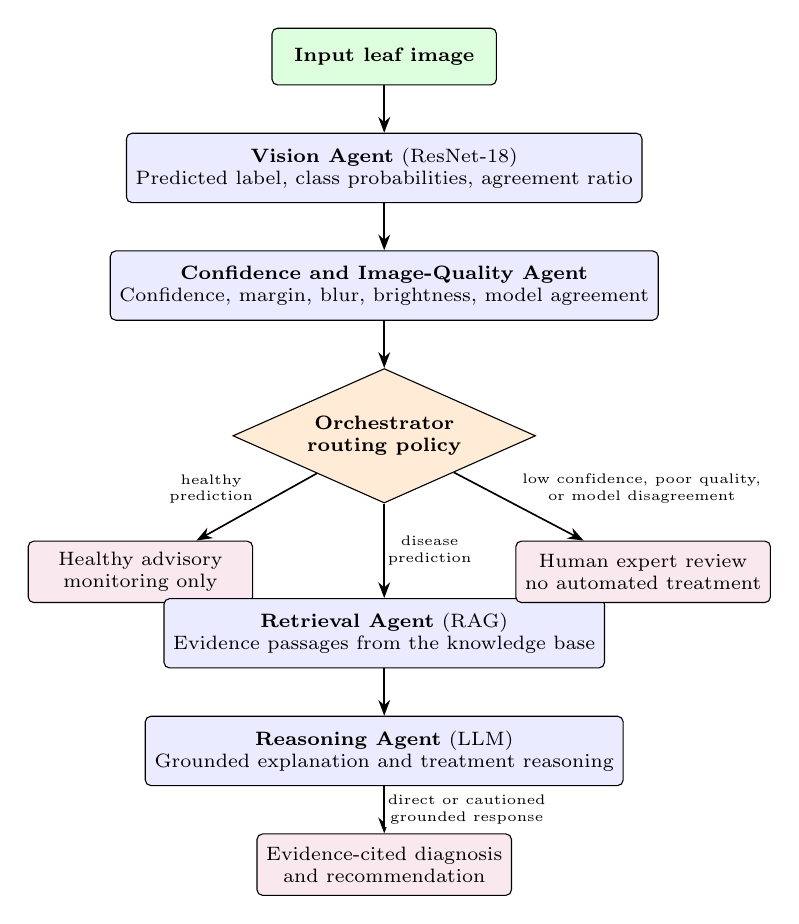
\begin{tikzpicture}[
  node distance=6mm and 9mm,
  input/.style={draw, rounded corners=2pt, minimum width=2.85cm, minimum height=0.72cm, align=center, font=\scriptsize\bfseries, fill=green!13},
  agent/.style={draw, rounded corners=2pt, minimum width=3.25cm, minimum height=0.88cm, align=center, font=\scriptsize, fill=blue!8},
  decision/.style={draw, diamond, aspect=2.25, minimum width=2.55cm, minimum height=0.95cm, align=center, font=\scriptsize\bfseries, fill=orange!16},
  outcome/.style={draw, rounded corners=2pt, minimum width=2.85cm, minimum height=0.78cm, align=center, font=\scriptsize, fill=purple!9},
  arrow/.style={-Stealth, semithick},
  label/.style={font=\tiny, align=center, fill=white, inner sep=1pt}
]
\node[input] (img) {Input leaf image};
\node[agent, below=of img] (vision) {\textbf{Vision Agent} (ResNet-18)\\Predicted label, class probabilities, agreement ratio};
\node[agent, below=of vision] (confidence) {\textbf{Confidence and Image-Quality Agent}\\Confidence, margin, blur, brightness, model agreement};
\node[decision, below=of confidence] (orch) {Orchestrator\\routing policy};
\node[outcome, below left=9mm and 7mm of orch] (healthy) {Healthy advisory\\monitoring only};
\node[agent, below=12mm of orch] (retrieval) {\textbf{Retrieval Agent} (RAG)\\Evidence passages from the knowledge base};
\node[agent, below=of retrieval] (reason) {\textbf{Reasoning Agent} (LLM)\\Grounded explanation and treatment reasoning};
\node[outcome, below=of reason] (recommendation) {Evidence-cited diagnosis\\and recommendation};
\node[outcome, below right=9mm and 7mm of orch] (human) {Human expert review\\no automated treatment};

\draw[arrow] (img) -- (vision);
\draw[arrow] (vision) -- (confidence);
\draw[arrow] (confidence) -- (orch);
\draw[arrow] (orch) -- node[label, above left]{healthy\\prediction} (healthy);
\draw[arrow] (orch) -- node[label, right]{disease\\prediction} (retrieval);
\draw[arrow] (retrieval) -- (reason);
\draw[arrow] (reason) -- node[label, right]{direct or cautioned\\grounded response} (recommendation);
\draw[arrow] (orch) -- node[label, above right]{low confidence, poor quality,\\or model disagreement} (human);
\end{tikzpicture}
\caption{Proposed agentic architecture for plant-disease diagnosis. The Orchestrator uses the prediction and reliability signals to route healthy cases to monitoring, disease cases through evidence retrieval and grounded reasoning, and unreliable cases to human review.}
\label{fig:arch}
\end{figure*}
\subsection{Vision Agent}
The Vision Agent processes an input leaf image with one or more ResNet-18 convolutional neural networks and returns a probability distribution over the PlantVillage disease taxonomy \cite{r_hughes2015,r_he2016}. The system supports a single ResNet-18 configuration and an ensemble of three checkpoints trained using Federated Averaging (FedAvg) \cite{r_fedavg}, Federated Optimization (FedOpt) \cite{r_fedopt}, and Federated Matched Averaging (FedMA) \cite{r_fedma}. 

\subsection{Confidence and Image-Quality Agent}
The Confidence and Image-Quality Agent performs lightweight, non-parametric post-processing on both the input image and the Vision Agent output. Rather than generating a new prediction, it produces a structured reliability signal using four measures: (i) \emph{confidence}, defined as the top-1 softmax probability; (ii) \emph{margin}, the difference between the top-1 and top-2 class probabilities; (iii) a binary \emph{quality flag}, obtained from a Laplacian-variance blur check and brightness-range check; and (iv), in ensemble mode, the \emph{agreement ratio}, which identifies disagreement among independently trained models even when averaged confidence is high. These signals are combined and forwarded to the Orchestrator.

\subsection{Retrieval Agent}
The Retrieval Agent implements retrieval-augmented generation (RAG) \cite{r_lewis2020} over a static knowledge base curated from publicly available agricultural-extension and plant-pathology reference materials. Given a predicted disease label and, when the prediction margin is low, its runner-up candidate, the agent returns the top-$k$ most relevant passages as grounding evidence for the Reasoning Agent.

\subsection{Reasoning Agent}
The Reasoning Agent is a large language model that receives the predicted disease label, its confidence and margin, and the passages returned by the Retrieval Agent. It produces three outputs: (i) a diagnosis statement identifying the most likely disease and, when the margin is low, up to two plausible alternatives; (ii) an explanation in which each factual claim is supported by a cited retrieved passage; and (iii) treatment and prevention recommendations derived from the retrieved evidence rather than unverified parametric knowledge.

\subsection{Orchestrator}
The Orchestrator makes the framework agentic by deciding which agents are activated for each case rather than applying a fixed pipeline. Its routing policy is summarized in Table~\ref{tab:policy}. 

\begin{table}[t]
\centering
\caption{Orchestrator Routing Policy}
\label{tab:policy}
\small
\begin{tabular}{p{3.6cm}p{3.6cm}}
\toprule
\textbf{Condition} & \textbf{Action} \\
\midrule
Healthy prediction & Monitoring advisory; retrieval and reasoning skipped (no treatment needed) \\
Disease, high confidence, high margin, model agreement, good image quality & Full pipeline: retrieval $\rightarrow$ reasoning $\rightarrow$ direct grounded, evidence-cited treatment \\
Disease, moderate confidence, or low margin, good image quality & Full pipeline: same grounded recommendation, with explicit alternatives and caveats \\
Low confidence, poor image quality, or heavy model disagreement & Escalate to human expert; no automated recommendation issued \\
\bottomrule
\end{tabular}
\end{table}

Algorithm~\ref{alg:orch} formalizes this routing logic.

\begin{algorithm}[t]
\caption{Orchestrator Routing Policy}
\label{alg:orch}
\begin{algorithmic}[1]
\REQUIRE image $x$; thresholds $\tau_{high}=0.85$, $\tau_{low}=0.55$, $\tau_{margin}=0.15$, $\tau_{agree}=0.5$
\STATE $\hat{y}, p, a \leftarrow \text{VisionAgent}(x)$ \COMMENT{label, softmax vector, agreement ratio}
\STATE $c \leftarrow \max(p)$; \ $m \leftarrow p_{(1)} - p_{(2)}$ \COMMENT{confidence, margin}
\STATE $q \leftarrow \text{QualityCheck}(x)$ \COMMENT{blur / brightness check}
\IF{$\hat{y}$ is healthy}
    \STATE \textbf{return} HealthyAdvisory($\hat{y}$) \COMMENT{no treatment; skip retrieval \& reasoning}
\ELSIF{$c < \tau_{low}$ \OR $a < \tau_{agree}$ \OR $q \neq \text{good}$}
    \STATE \textbf{return} EscalateToHuman($x, \hat{y}, c, q, a$)
\ELSE
    \STATE $D \leftarrow \text{RetrievalAgent}(\hat{y})$ \COMMENT{ground every disease diagnosis}
    \STATE $r \leftarrow \text{ReasoningAgent}(\hat{y}, c, m, D)$
    \IF{$c \geq \tau_{high}$ \AND $m \geq \tau_{margin}$ \AND $a = 1$}
        \STATE \textbf{return} DirectDiagnosis($r$) \COMMENT{confident grounded recommendation}
    \ELSE
        \STATE \textbf{return} CautionedDiagnosis($r$) \COMMENT{grounded, with alternatives/caveats}
    \ENDIF
\ENDIF
\end{algorithmic}
\end{algorithm}

\section{Implementation Details}
\label{sec:impl}

\textbf{Dataset.} We used the PlantVillage dataset \cite{r_hughes2015}, which comprises leaf images from multiple crop species and disease categories. The data are divided into training, validation, and held-out test partitions using the split from our prior federated-learning experiments.

\textbf{Vision backbone.} The ResNet-18 model \cite{r_he2016} from our previous work is reused without modification, allowing this study to isolate the contribution of the agentic layer. We evaluate two Vision Agent configurations: a single checkpoint trained with FedAvg, and a three-model ensemble combining checkpoints trained with FedAvg, FedOpt, and FedMA. The ensemble averages the softmax outputs to produce the final prediction. All checkpoints use the same 38-class ResNet-18 architecture and differ only in their federated aggregation strategy.

\textbf{Orchestrator thresholds.} The high-confidence, low-confidence, and margin thresholds are set to 0.85, 0.55, and 0.15, respectively. In ensemble mode, an agreement-ratio threshold of 0.5 identifies cases in which the member models substantially disagree. These thresholds bias the system toward caution: when confidence, margin, or inter-model agreement falls outside the conservative operating range, the case is escalated for human review rather than handled autonomously.

\textbf{Retrieval index.} Reference documents are divided into smaller chunks and embedded with the \texttt{bge-small-en-v1.5} sentence-embedding model. The embeddings are stored in a FAISS vector store \cite{r_faiss} for cosine-similarity retrieval, and the Retrieval Agent returns the top-$k$ relevant passages for each query, with $k=5$.

\textbf{Reasoning model.} The Reasoning Agent uses an instruction-tuned large language model accessed through an OpenAI-compatible API and a provider-agnostic wrapper. This design permits the language model to be replaced without changing the remainder of the system. A fixed prompt template requires a passage-grounded citation for each factual claim and instructs the model not to recommend a treatment unless it is supported by the retrieved evidence.

\textbf{Knowledge base.} The Retrieval Agent uses a static knowledge base comprising 125 curated documents drawn from open-access PubMed Central articles, agricultural-extension resources, and plant-pathology reference materials. These documents cover symptoms, causal pathogens, and management practices for the crop-disease categories in the PlantVillage taxonomy. After chunking and embedding, the knowledge base contains 16{,}706 indexed passage chunks, enabling passage-level rather than document-level evidence retrieval.

\textbf{Episodic logging.} Each case handled by the Orchestrator, together with its routing decision and final output, is stored in a structured record. These records are used for offline evaluation (Section~\ref{sec:exp}) and provide a basis for a complete episodic Memory Agent in future work, as discussed in Section~\ref{sec:conclusion}.

\section{Experimental Setup}
\label{sec:exp}

We evaluated the system on two test datasets. The in-distribution PlantVillage dataset contains 114 held-out images, with three images from each of 38 crop-disease classes. These images are drawn from the same source used to train the Vision Agent. The out-of-distribution (OOD) Dataset contains 190 leaf images, with five images per class across the same 38 categories, collected from public web sources outside PlantVillage. Together, the two datasets assess same-source performance and generalization under uncontrolled photographic conditions. We reported results for the three individual models (FedAvg, FedOpt, and FedMA) and the three-model ensemble on both datasets, using classification and agentic metrics.

\textbf{Classification metrics.} We measure the Vision Agent's top-1 accuracy and macro-averaged F1 score to establish the baseline perceptual performance on which the agentic layer builds.

\textbf{Agentic metrics.} The Orchestrator assigns each case exactly one of three routes: a \emph{direct diagnosis} $D$ (high confidence), \emph{retrieve-and-reason} $R$ (moderate confidence; evidence is retrieved and the recommendation carries alternatives and caveats), or \emph{escalation} $E$ (deferred to a human). These metrics score the \emph{routing decision}. Let $D_{=}$ and $D_{\neq}$ be direct diagnoses with correct and incorrect predictions, and $E_{\neq}$ escalations with incorrect predictions. With $N$ test cases:
\begin{align}
\text{Correct-action rate} &= \frac{|D_{=}| + |R| + |E_{\neq}|}{N} \\
\text{Harmful-action rate} &= \frac{|D_{\neq}|}{N} \\
\text{Human-intervention rate} &= \frac{|E|}{N}
\end{align}
These rates are not a partition of $N$: an escalated case with a wrong underlying prediction counts both as a correct routing decision and as an intervention, so they need not sum to $100\%$. We additionally report the \emph{naive baseline harmful-action rate}, defined as the classifier's raw error rate under a policy that always acts regardless of confidence equivalent to deploying the Vision Agent alone without any orchestration. The reduction from this baseline to the agentic harmful-action rate is the primary indicator of the value added by the Confidence/Quality Agent and Orchestrator.

\textbf{Grounding check.} For cases processed through the full pipeline, we examine the reasoning outputs to determine whether each factual claim is supported by its cited retrieved passage and whether the system avoids treatments that are unsupported by the available evidence. A formal, large-scale grounding annotation with inter-annotator agreement is left for future work.

\textbf{Retrieval coverage.} We measure retrieval coverage as the fraction of the 38 classes for which the knowledge base returns at least one strongly relevant passage, defined by cosine similarity $\geq 0.75$, when queried by class name.
\section{Results and Discussion}
\label{sec:results}
We evaluated the in-distribution PlantVillage set and the OOD Dataset containing web-sourced images for each individual model and for the three-model ensemble. Fig.~\ref{fig:gap} compares top-1 accuracy across the two datasets, and Fig.~\ref{fig:safety} shows the safety improvement of the agentic layer on the OOD Dataset.

\begin{table}[H]
\centering
\caption{Classification results on held-out PlantVillage images (114 images, three per class across 38 classes). All values are percentages; best values are in bold.}
\label{tab:classification_id}
\small
\setlength{\tabcolsep}{8pt}
\begin{tabular}{lrr}
\toprule
\textbf{Configuration} & \textbf{Accuracy} & \textbf{Macro-F1} \\
\midrule
FedAvg & \textbf{99.1} & \textbf{99.0} \\
FedOpt & 95.6 & 95.3 \\
FedMA & 86.0 & 82.8 \\
\textbf{Ensemble} & \textbf{99.1} & \textbf{99.0} \\
\bottomrule
\end{tabular}
\end{table}

\begin{table}[H]
\centering
\caption{Agentic-safety results on held-out PlantVillage images. The proposed agentic system and naive classifier-only baseline are reported separately. All values are percentages; best values are in bold.}
\label{tab:safety_id}
\scriptsize
\setlength{\tabcolsep}{1.5pt}
\renewcommand{\arraystretch}{1.15}
\begin{tabular}{lcccc}
\toprule
& \multicolumn{3}{c}{\textbf{Proposed agentic system}} & \multicolumn{1}{c}{\shortstack{\textbf{Naive classifier-}\\\textbf{only baseline}}} \\
\cmidrule(lr){2-4}\cmidrule(l){5-5}
\textbf{Configuration} & \shortstack{\textbf{Correct-}\\\textbf{action rate}} & \shortstack{\textbf{Harmful-}\\\textbf{action rate}} & \shortstack{\textbf{Human-intervention}\\\textbf{rate}} & \shortstack{\textbf{Harmful-}\\\textbf{action rate}} \\
\midrule
FedAvg & \textbf{99.1} & \textbf{0.0} & 0.9 & \textbf{0.9} \\
FedOpt & 97.4 & 0.9 & 3.5 & 4.4 \\
FedMA & 87.7 & 3.5 & 17.5 & 14.0 \\
\textbf{Ensemble} & \textbf{99.1} & \textbf{0.0} & \textbf{0.9} & \textbf{0.9} \\
\bottomrule
\end{tabular}
\renewcommand{\arraystretch}{1}
\end{table}

\begin{table}[H]
\centering
\caption{Classification results on the OOD Dataset of web-sourced images (190 images, five per class across 38 classes). All values are percentages; best values are in bold.}
\label{tab:classification_ood}
\small
\setlength{\tabcolsep}{8pt}
\begin{tabular}{lrr}
\toprule
\textbf{Configuration} & \textbf{Accuracy} & \textbf{Macro-F1} \\
\midrule
FedAvg & 67.9 & 70.9 \\
FedOpt & 66.3 & 68.7 \\
FedMA & 61.1 & 60.0 \\
\textbf{Ensemble} & \textbf{68.4} & \textbf{71.1} \\
\bottomrule
\end{tabular}
\end{table}

\begin{table}[H]
\centering
\caption{Agentic-safety results on the OOD Dataset. The proposed agentic system and naive classifier-only baseline are reported separately. All values are percentages; best values are in bold.}
\label{tab:safety_ood}
\scriptsize
\setlength{\tabcolsep}{1.5pt}
\renewcommand{\arraystretch}{1.15}
\begin{tabular}{lcccc}
\toprule
& \multicolumn{3}{c}{\textbf{Proposed agentic system}} & \multicolumn{1}{c}{\shortstack{\textbf{Naive classifier-}\\\textbf{only baseline}}} \\
\cmidrule(lr){2-4}\cmidrule(l){5-5}
\textbf{Configuration} & \shortstack{\textbf{Correct-}\\\textbf{action rate}} & \shortstack{\textbf{Harmful-}\\\textbf{action rate}} & \shortstack{\textbf{Human-intervention}\\\textbf{rate}} & \shortstack{\textbf{Harmful-}\\\textbf{action rate}} \\
\midrule
FedAvg & \textbf{86.8} & 11.1 & \textbf{15.8} & 32.1 \\
FedOpt & 85.8 & 10.5 & 20.5 & 33.7 \\
FedMA & 82.1 & \textbf{6.8} & 38.9 & 38.9 \\
\textbf{Ensemble} & \textbf{86.8} & \textbf{6.8} & 28.4 & \textbf{31.6} \\
\bottomrule
\end{tabular}
\renewcommand{\arraystretch}{1}
\end{table}

\textbf{PlantVillage and OOD performance.}  On the in-distribution PlantVillage images (Table~\ref{tab:classification_id}), individual models attain 86.0--99.1\% top-1 accuracy and the ensemble matches the best single model at 99.1\%. On the OOD Dataset (Table~\ref{tab:classification_ood}), individual models attain 61.1--67.9\% top-1 accuracy and the ensemble attains 68.4\%, as shown in Fig.~\ref{fig:gap}.


\textbf{Comparison to a classifier-only baseline.} Mohanty et al.~\cite{r_mohanty2016} report 99.35\% on held-out PlantVillage but 31.40\% on 121 web-sourced images spanning the same 38 classes, and act on every prediction, and do not use any quality or confidence agent; therefore every wrong prediction leads to harmful advice, giving a harmful-action rate of $100-31.40=68.60\%$ (Figs.~\ref{fig:gap} and~\ref{fig:safety}). Because each study collected its own web-sourced set, these figures indicate the magnitude of the domain gap reported by each study rather than a controlled head-to-head comparison.

\textbf{Value of the agentic layer.} The safety tables (Tables~\ref{tab:safety_id} and~\ref{tab:safety_ood}) distinguish the proposed agentic system from the naive classifier-only baseline. On the OOD Dataset, the naive baseline has a harmful-action rate of 31.6--38.9\% across the four configurations (Table~\ref{tab:safety_ood}), whereas the proposed agentic system reduces this rate to 6.8--11.1\%. For the ensemble, harmful actions decrease from 31.6\% under the naive baseline to 6.8\% under the proposed agentic system, while 28.4\% of cases are escalated to a human expert in our proposed system. 

\textbf{Single model versus ensemble.} On the OOD Dataset, the ensemble achieves the highest top-1 accuracy (68.4\%) and macro-F1 score (71.1\%) in Table~\ref{tab:classification_ood}. In Table~\ref{tab:safety_ood}, its correct-action rate of 86.8\% ties the FedAvg result, and its harmful-action rate of 6.8\% ties the lowest value. The ensemble also has the lowest naive-baseline harmful-action rate (31.6\%). In ensemble mode, agreement among the three member models provides more confidence in the prediction, since a prediction is more likely to be correct when more than one model agrees on it, and therefore supplies an additional signal for the Orchestrator's deferral decision alongside confidence, margin, and image quality.

\begin{figure}[H]
    \centering
    \includegraphics[width=\columnwidth]{fig_baseline_accuracy.png}
    \caption{Top-1 accuracy on held-out PlantVillage images and the OOD Dataset of web-sourced images, for the classifier-only baseline of Mohanty et al.~\cite{r_mohanty2016} and for each configuration of this work. Both evaluate the same 38-class taxonomy, but each study collected its own web-sourced OOD set (121 images in~\cite{r_mohanty2016}; 190 here).}
    \label{fig:gap}
\end{figure}


\begin{figure}[H]
    \centering
    \includegraphics[width=\columnwidth]{fig_baseline_safety.png}
    \caption{Safety improvement on the OOD Dataset: the fraction of cases receiving harmful (incorrect) automated advice under the naive classifier-only baseline versus the proposed agentic system, which defers uncertain cases to a human. The baseline of Mohanty et al.~\cite{r_mohanty2016} performs no uncertainty-based escalation, so its harmful-action rate equals its error rate ($100-31.40=68.60\%$) and no agentic bar is defined for it.}
    \label{fig:safety}
\end{figure}

\textbf{Grounding and coverage.} Retrieval coverage is complete: all 38 classes return strongly relevant passages from the knowledge base. Qualitative inspection of the full-pipeline reasoning outputs found that they cite specific retrieved passages for their factual claims and, when the retrieved evidence described symptoms but lacked treatment guidance, the Reasoning Agent declined to fabricate a treatment and instead recommended expert consultation, which is the intended hallucination-averse behavior. Because the Orchestrator skips retrieval and reasoning for healthy plants and for escalated cases (those referred to human experts), the LLM is invoked only for the disease diagnoses where a grounded treatment is actually actionable, incurring lower average inference cost than a design that reasons over every input.


\FloatBarrier

\section{Conclusion and Future Work}
\label{sec:conclusion}

The paper presented an agentic AI framework that upgrades a standard CNN-based plant disease classifier into an autonomous, explainable, and safety-aware diagnostic advisory system. By decomposing the diagnostic process into a Vision Agent, a Confidence and Image-Quality Agent, a Retrieval Agent, a Reasoning Agent, and an Orchestrator that conditions computation and action on predictive uncertainty, the system moves beyond single-shot classification toward the autonomy, goal-directed reasoning, and environment-aware deferral that characterize agentic AI. 


\bibliographystyle{IEEEtran}
\bibliography{references}


\end{document}